\chapter{Transformations linéaires}

% need to draw shapes *underneath* everything...
\newcommand{\CoordInitiales}{% les 4 points point: coordonnées
	\coordinate (A0) at (0, 0);
	\coordinate (B0) at (0, 1);
	\coordinate (C0) at (1, 0);
	\coordinate (D0) at (1, 1);
}% end of \CoordInitiales

\newcommand{\DessinerAxes}{
	% les axes
	\draw[->] (-1.5,0) -- (2.5,0) node[anchor=west]{x};
	\draw[->] (0,-1.5) -- (0,2.5) node[anchor=south]{y};
	% tick marks
	\draw[-] (1, -0.1) node[anchor=north]{\tiny 1} -- (1, 0.1);
	\draw[-] (-0.1, 1) node[anchor=east]{\tiny 1} -- (0.1, 1);
	\draw[-] (-1, -0.1) node[anchor=north]{\tiny -1} -- (-1, 0.1);
	\draw[-] (-0.1, -1) node[anchor=east]{\tiny -1} -- (0.1, -1);
	\draw[-] (2, -0.1) node[anchor=north]{\tiny 2} -- (2, 0.1);
	\draw[-] (-0.1, 2) node[anchor=east]{\tiny 2} -- (0.1, 2);
	% les 4 points point: drawing on top
	\draw [black] (A0) circle (2pt);
	\draw [red] (B0) circle (2pt);
	\draw [green] (C0) circle (2pt);
	\draw [blue] (D0) circle (2pt);
}% end of \DessinerAxes

\newcommand{\FigureInitiale}{
\CoordInitiales
% initial area
\path [fill=blue!10] (A0) -- (B0) -- (D0) -- (C0) -- (A0);
\DessinerAxes
}

\newcommand{\FigureFinale}{
    %%%% Remember to first define the final coordinates (A) through (D)
    \CoordInitiales
    % initial area
    \path [fill=blue!10] (A0) -- (B0) -- (D0) -- (C0) -- (A0);
    % final area
    \path [pattern=north east lines, pattern color=blue] (A) -- (B) -- (D) -- (C) -- (A);
    \DessinerAxes
	% les 4 points point: drawing on top
	\fill [black] (A) circle (2pt);
	\fill [red] (B) circle (2pt);
	\fill [green] (C) circle (2pt);
	\fill [blue] (D) circle (2pt);
}
\section{Introduction}
Dans le chapitre précédent, nous avons vu les espaces vectoriels et démontrés comment ils
étaient isomorphes à $\BBR^n$.  Dans ce chapitre nous allons considérer certaines
propriétés des fonctions sur les espaces vectoriels. Pour illustrer ceci, et sans perte de généralité,
nous allons considérer $\BBR^n$ comme espace vectoriel.
\begin{defini}
Une \Definition{transformation} (ou \textbf{fonction} ou \textbf{application}) $T$ de $\BBR^n$ 
(le domaine de définition) vers $\BBR^m$ (le \Definition{codomaine}, ou ensemble d'arrivée)
est une règle qui associe à chaque vecteur $\mat{v}$ de $\BBR^n$ un vecteur $\mat{u} = T(\mat{v})$ de $\BBR^m$.
De façon résumée, on écrit parfois ceci comme 
$
T: \BBR^n \rightarrow \BBR^m
$
\end{defini}

Pour chaque $\mat{v}$ dans $\BBR^n$, on dit de $T(\mat{v})$ que c'est l'\definition{image} de $\mat{v}$. 
L'ensemble de toutes les images $T(\mat{v})$ est appelé l'image de la transformation $T$, ou tout simplement l'image de $T$.

\begin{defini}
Une transformation $T$ est une \Definition{transformation linéaire} si, pour
tout $\mat{u}, \mat{v}$ dans le domaine de $T$:
\begin{enumerate}
\item $T(\mat{u}+\mat{v}) = T(\mat{u}) + T(\mat{v})$
\item $T(c\mat{v}) = cT(\mat{v})$, où $c$ est un scalaire.
\end{enumerate}
\end{defini}

On peut résumer ces deux propriétés en une seule, tel que démontré dans le théorème suivant.
\pagebreak


\begin{theo}
Soit $T$  une transformation de $\BBR^n$ vers $\BBR^m$.  La transformation $T$
est linéaire si et seulement si
\[
T(c\mat{u} + d\mat{v}) = cT(\mat{u}) + dT(\mat{v})
\]
quels que soient les vecteurs $\mat{u}$ et $\mat{v}$ dans le domaine de définition
de $T$ et quels que soient les scalaires $c$ et $d$.
\proof
Si $T$ est une transformation linéaire, alors, en appliquant successivement les propriétés
1 et 2, nous avons
\[
T(c\mat{u} + d\mat{v}) = T(c\mat{u}) + T(d\mat{v}) = cT(\mat{u}) + dT(\mat{v})
\]
Inversement, si 
\[
T(c\mat{u} + d\mat{v}) = cT(\mat{u}) + dT(\mat{v})
\]
en choisissant $c=d=1$, nous obtenons la première propriété, et en choisissant $d=0$, nous
obtenons la deuxième.
\end{theo}
On remarque que nous avons également $T(\zero) = \zero$, en choississant $c=0$ dans la deuxième propriété
de la définition d'une transformation linéaire.


\begin{defini}
Une \Definition{transformation matricielle} est une transformation $T$ qui est calculée par
le produit matriciel
$
\mat{M}\mat{v} = \mat{u}
$
où $\mat{M}$ est une matrice $m\times n$.
\end{defini}

En raison des propriétés des matrices, toutes les transformations matricielles sont des transformations linéaires.
\begin{exerciceB}
Prouvez que toutes les transformations matricielles sont des transformations linéaires.
\end{exerciceB}

Si la matrice $\mat{M}$ d'une transformation linéaire a $n$ colonnes, le domaine de définition est $\BBR^n$.
Si la matrice $\mat{M}$ d'une transformation linéaire a $m$ lignes, le codomaine est un sous-ensemble $\BBR^m$.

\begin{exemple}
Exemple de transformation matricielle $T: \BBR^4 \rightarrow\BBR^2$
\[
\begin{pmatrix}
1 & 2 & 3 & 4 \\
5 & 6 & 7 & 8
\end{pmatrix}
\begin{pmatrix}
1 \\ 2 \\ 3 \\ 4
\end{pmatrix}
=
\begin{pmatrix}
30 \\
70
\end{pmatrix}
\]
\end{exemple}

\begin{theo}
Soit $T: \BBR^n \rightarrow\BBR^m$ une transformation linéaire.  Il existe une
matrice unique, $\mat{M}$, appelée la \Definition{matrice canonique} de la transformation, 
telle que $T(\mat{x}) = \mat{M}\mat{x}$ pour tout $\mat{x}\in\BBR^n$.
\proof
Si on choisit la base canonique comme étant l'ensemble des colonnes de $I_n$, et donc
$I_n = ( \mat{e}_1 \cdots \mat{e}_n)$, on a
\[
\mat{x} = I_n\mat{x} = x_1\mat{e}_1 + \cdots + x_n \mat{e}_n
\]
Utilisant la linéarité de $T$, on a
\begin{eqnarray*}
T(\mat{x}) &=& T( x_1\mat{e}_1 + \cdots + x_n \mat{e}_n ) \\
  &=& x_1T(\mat{e}_1) + \cdots + x_nT(\mat{e}_n) \\
  &=& \displaystyle [\underbrace{T(\mat{e}_1) \cdots T(\mat{e}_n)]}_{\color{blue}\mat{M}} \begin{pmatrix}[c]
  x_1 \\
  \vdots\\
  x_n
  \end{pmatrix}\\
  = \mat{M}\mat{x}
\end{eqnarray*}
\end{theo}

\section{Transformation du plan}
Nous allons tout d'abord considérer les transformations
du plan, c'est-à-dire $\BBR^2 \rightarrow \BBR^2$. 
\[
\mat{M}\begin{pmatrix}
x \\ y
\end{pmatrix} = \begin{pmatrix}
x' \\ y'
\end{pmatrix}
\]
Notre but, en faisant ceci, est de donner des exemples simples
où les calculs sont faciles à suivre et où il est facile d'illustrer
l'effet des transformations.  Graphiquement, nous allons généralement considérer
une seule configuration initiale de quatre points formant un carré et démontrer
l'effet de la transformation sur ces quatre points, ainsi que sur l'aire de la figure
qu'ils composent. 

%%%%%%%%%%%%%%%%%%%%%%%%%%%%%%%%%%%%%%%%%%%%%%%
\begin{figure}[h]
\begin{minipage}{0.45\textwidth}
	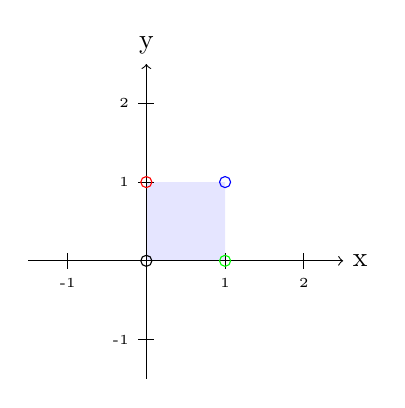
\begin{tikzpicture}
	\FigureInitiale
	\end{tikzpicture}
\caption{Figure initiale.}
\end{minipage}
\hfill
\begin{minipage}{0.45\textwidth}
	\begin{tikzpicture}
	% les 4 points point: coordonnées
	\coordinate (A) at (1.5, 0.5);
	\coordinate (B) at (1.8, 1.5);
	\coordinate (C) at (2.5, 0.5);
	\coordinate (D) at (2.8, 1.5);
	\FigureFinale
	\end{tikzpicture}
\caption{La figure initiale, en bleu pale, est transformée et
représentée en bleu foncé hachuré.}
\label{fig:nonlin}
\end{minipage}
\end{figure}
%%%%%%%%%%%%%%%%%%%%%%%%%%%%%%%%%%%%%%%%%%%%%%

Pour les transformations linéaires du plan, la matrice la plus générale\footnote{
Il est facile de vérifier qu'une telle transformation linéaire fait en sorte que le vecteur
nul, $\transp{(0, 0)}$, ne changera pas.  Par conséquent, la figure \ref{fig:nonlin} ne
représente pas une transformation linéaire du plan; c'est une transformation affine.}
 a la forme
\[
\mat{M} = \begin{pmatrix}
a & b \\
c & d
\end{pmatrix}
\]
Parmi toutes les combinaisons possibles, nous allons maintenant considérer quelques cas particuliers.
Veuillez noter que l'on peut combiner des transformations linéaires: il suffit de multiplier les
matrices correspondant aux transformations individuelles.

\subsection{Changements d'échelle: dilatation et contraction}

Une transformation linéaire du plan peut résulter en un changement d'échelle, soit une contraction ou une dilatation,
si la matrice de transformation est une matrice diagonale, avec des éléments positifs sur la diagonale:
\[
\mat{M} =\begin{pmatrix}[cc]
d_1 & 0 \\
0 & d_2
\end{pmatrix}
, \qquad d_i > 0
\]

\begin{figure}
\fbox{
\begin{minipage}{0.45\textwidth}
	\begin{tikzpicture}
	% les 4 points point: coordonnées
	\coordinate (A) at (0, 0);
	\coordinate (B) at (0, 2);
	\coordinate (C) at (2, 0);
	\coordinate (D) at (2, 2);
    \FigureFinale
	\end{tikzpicture}
\caption{Dilatation.}\[
\begin{pmatrix}
2 & 0 \\
0 & 2
\end{pmatrix}\begin{pmatrix}
x\\y
\end{pmatrix}=\begin{pmatrix}
2x\\2y
\end{pmatrix}
\]
\end{minipage}
}
\hfill
\fbox{
\begin{minipage}{0.45\textwidth}
	\begin{tikzpicture}
	% les 4 points point: coordonnées
	\coordinate (A) at (0, 0);
	\coordinate (B) at (0, 2);
	\coordinate (C) at (0.5, 0);
	\coordinate (D) at (0.5, 2);
    \FigureFinale
	\end{tikzpicture}
\caption{Dilatation verticale et contraction horizontale}
\[
\begin{pmatrix}
\frac{1}{2} & 0 \\
0 & 2
\end{pmatrix}\begin{pmatrix}
x\\y
\end{pmatrix}=\begin{pmatrix}
\frac{1}{2}x\\2y
\end{pmatrix}
\]
\end{minipage}
}
\end{figure}

%%%%%%%%%%%%%%%%%%%%%%%%%%%%%%%%%%%%%%%%%%%%%%%
\subsection{Cisaillement}
Une matrice correspondant à une transformation de \definition{cisaillement horizontal}
a la forme
\[
\mat{M} = \begin{pmatrix}
1 & k \\
0 & 1
\end{pmatrix}
\]
De la même façon, une matrice correspondant à une transformation de \definition{cisaillement vertical} 
a la forme
\[
\mat{M} = \begin{pmatrix}
1 & 0 \\
k & 1
\end{pmatrix}
\]
%%%%%%%%%%%%%%%%%%%%%%%
\begin{figure}[h]
\fbox{
\begin{minipage}{0.45\textwidth}
	\begin{tikzpicture}
	% les 4 points point: coordonnées
	\coordinate (A) at (0, 0);
	\coordinate (B) at (1.5, 1);
	\coordinate (C) at (1, 0);
	\coordinate (D) at (2.5, 1);
    \FigureFinale
	\end{tikzpicture}
\caption{Cisaillement horizontal}\[
\begin{pmatrix}
1 & 1\frac{1}{2} \\
0 & 1
\end{pmatrix}\begin{pmatrix}
x\\y
\end{pmatrix}=\begin{pmatrix}[c]
x + 1\frac{1}{2}y\\y
\end{pmatrix}
\]
\end{minipage}
}
\hfill
\fbox{
\begin{minipage}{0.45\textwidth}
	\begin{tikzpicture}
	% les 4 points point: coordonnées
	\coordinate (A) at (0, 0);
	\coordinate (B) at (-.707, 0.707);
	\coordinate (C) at (.707, 0.707);
	\coordinate (D) at (0, 1.414);
    \FigureFinale
	\end{tikzpicture}
\caption{Rotation de $\pi/4$.}
\[
\begin{pmatrix}
\frac{\sqrt{2}}{2} &\frac{-\sqrt{2}}{2} \\
\frac{\sqrt{2}}{2} & \frac{\sqrt{2}}{2}
\end{pmatrix}\begin{pmatrix}
x\\y
\end{pmatrix}=\begin{pmatrix}
\frac{\sqrt{2}}{2}x - \frac{\sqrt{2}}{2}y\\
\frac{\sqrt{2}}{2}x + \frac{\sqrt{2}}{2}y
\end{pmatrix}
\]
\end{minipage}
}
\end{figure}
%%%%%%%%%%%%%%%%%%%%%%%%%%%%%%%%%%

\subsection{Rotation}
Une matrice correspondant à une rotation d'un angle $\theta$ des axes autour de l'origine a la forme
\[
\mat{R}(\theta) = \begin{pmatrix}
\cos\theta & -\sin\theta \\
\sin\theta & \cos\theta
\end{pmatrix}
\]
Notez que, par convention, on utilise habituellement la lettre $\mat{R}$ pour dénoter des rotations.


\subsection{Réflexion}
La matrice correspondant à une réflexion par rapport à l'axe vertical
est la matrice:
\[
\mat{M} = \begin{pmatrix}
-1 & 0 \\
0 & 1
\end{pmatrix} 
\]
La matrice correspondant à une réflexion par rapport à l'axe horizontal
est la matrice:
\[
\mat{M} = \begin{pmatrix}
1 & 0 \\
0 & -1
\end{pmatrix} 
\]

%%%%%%%%%%%%%%%%%%%%%%%%%%%%%%%%%%%%%%%%%%%%%%%
\begin{figure}[h]
\fbox{
\begin{minipage}{0.45\textwidth}
	\begin{tikzpicture}
	% les 4 points point: coordonnées
	\coordinate (A) at (0, 0);
	\coordinate (B) at (0, 1);
	\coordinate (C) at (-1, 0);
	\coordinate (D) at (-1, 1);
    \FigureFinale
	\end{tikzpicture}
\caption{Réflexion par rapport à l'axe des $y$.}
\[
\begin{pmatrix}
-1 & 0 \\
0 & 1
\end{pmatrix}\begin{pmatrix}
x\\y
\end{pmatrix}=\begin{pmatrix}
-x\\y
\end{pmatrix}
\]
\end{minipage}
}
\hfill
\fbox{
\begin{minipage}{0.45\textwidth}
	\begin{tikzpicture}
	% les 4 points point: coordonnées
	\coordinate (A) at (0, 0);
	\coordinate (B) at (0, -1);
	\coordinate (C) at (-1, 0);
	\coordinate (D) at (-1, -1);
    \FigureFinale
	\end{tikzpicture}
\caption{Réflexion par rapport aux deux axes.}
\[
\begin{pmatrix}
-1 & 0 \\
0 & -1
\end{pmatrix}\begin{pmatrix}
x\\y
\end{pmatrix}=\begin{pmatrix}
-x\\-y
\end{pmatrix}
\]
\end{minipage}
}
\end{figure}
%%%%%%%%%%%%%%%%%%%%%%%%%%%%%%%%%%%%%%%%%%%%%%%


\subsection{Combinaison de transformations}

En faisant des combinaisons de transformations simples, on peut arriver à en créer
des complexes.  L'exemple le plus simple est possiblement celui de la
matrice $-\matI$, qui correspond à une réflexion par rapport aux deux axes ce qui peut
être vu comme une première réflexion faite par rapport à l'axe horizontal, suivie
par une deuxième réflexion, faite par rapport à l'axe vertical.  Veuillez noter
que le résultat n'est pas le même que si nous avions fait une seule réflexion
par rapport à la droite $y=-x$.

\begin{exerciceB}
Trouvez la matrice qui correspond à une réflexion par rapport à la droite
$y=-x$.  Faites un diagramme qui illustre ceci.
\end{exerciceB}

Un exemple un peu plus intéressant est celui d'une réflexion par rapport à un
axe quelconque passant par l'origine\footnote{La raison pour laquelle
on mentionne que l'axe passe par l'origine est pour que l'on ait 
$T(\zero) = \zero$ ce qui est requis pour que la transformation soit linéaire.}.
Pour produire une réflexion par rapport à un axe quelconque passant par l'origine, vous
devriez pouvoir vous convaincre qu'il suffit de suivre la procédure suivante.
\begin{enumerate}
\item Déterminer l'angle $\theta$ que fait l'axe par rapport à l'axe horizontal.
\item Faire une rotation de $-\theta$.
\item Faire une réflexion par rapport à l'axe horizontal
\item Faire une rotation de $\theta$ pour revenir à l'orientation initiale.
\end{enumerate}
Comme ceci correspond à trois transformations, la transformation peut être exprimée sous
la forme d'un produit de trois matrices comme suit:
\[
\begin{pmatrix}
\cos\theta & -\sin\theta \\
\sin\theta & \cos\theta
\end{pmatrix}
\begin{pmatrix}
1 & 0 \\
0 & -1
\end{pmatrix}
\begin{pmatrix}
\cos\theta & \sin\theta \\
-\sin\theta & \cos\theta
\end{pmatrix}
=
\begin{pmatrix}[cc]
\cos^2\theta-\sin^2\theta & 2\sin\theta \cos\theta \\
2\sin\theta\cos\theta & \sin^2\theta-\cos^2\theta
\end{pmatrix}
\]
À noter que l'ordre des opérations est de droite à gauche!

\subsection{Projections}
Les projections dans le plan consistent à calculer la composante d'un vecteur
selon un axe et de lui donner cette valeur.  Le cas le plus simple est
celui de la projection sur l'axe des $x$ (ou, de façon semblable, sur l'axe
des $y$):
\[
\begin{pmatrix}
1 & 0 \\
0 & 0
\end{pmatrix}
\begin{pmatrix}
x \\ y
\end{pmatrix}
= \begin{pmatrix}
x\\0
\end{pmatrix}
\]
Ce type de transformation linéaire n'est pas inversible: une fois la projection
sur l'axe des $x$ effectuée, nous perdons toute connaissance de la valeur
initiale de la coordonnée $y$, et donc, nous ne pouvons pas la retrouver.

Une autre façon d'exprimer ceci est de noter que la matrice qui effectue
la projection n'a pas d'inverse.
%%%%%%%%%%%%%%%%%%%%%%%%%%%%%%%%%%%%
\begin{figure}
\fbox{
\begin{minipage}{0.45\textwidth}
	\begin{tikzpicture}
	% les 4 points point: coordonnées
	\coordinate (A) at (0, 0);
	\coordinate (B) at (0, 0);
	\coordinate (C) at (1, 0);
	\coordinate (D) at (1, 0);
    \FigureFinale
	\end{tikzpicture}
\caption{Projection sur l'axe des $x$. Les points noir et rouge sont confondus, ainsi que
les points bleu et vert.}
\[
\begin{pmatrix}
1 & 0 \\
0 & 0
\end{pmatrix}\begin{pmatrix}
x\\y
\end{pmatrix}=\begin{pmatrix}
x\\0
\end{pmatrix}
\]
\end{minipage}
}
\hfill
\fbox{
\begin{minipage}{0.45\textwidth}
	\begin{tikzpicture}
	% les 4 points point: coordonnées
	\coordinate (A) at (0, 0);
	\coordinate (B) at (0.5, 0.5 );
	\coordinate (C) at (0.5, 0.5);
	\coordinate (D) at (1, 1);
    \FigureFinale
    \draw[blue] (A) -- (D);
	\end{tikzpicture}
\caption{Projection sur la droite $y=x$. Les points rouge et vert sont confondus et le carré
est devenu un segment de droite.}
\[
\frac{1}{2}\begin{pmatrix}
1 &1 \\
1 & 1
\end{pmatrix}\begin{pmatrix}
x\\y
\end{pmatrix}=\frac{1}{2}\begin{pmatrix}
x+y\\x+y
\end{pmatrix}
\]
\end{minipage}
}
\end{figure}

\section{Translations}
Une translation est une transformation qui correspond à l'addition d'un vecteur constant à tous les vecteurs d'un domaine: $T(\mat{x}) = \mat{x} + \mat{x}_0$.
Une telle transformation n'est pas une transformation linéaire: $T\mat{\zero} \neq \zero$ sauf dans le cas trivial où $\mat{x}_0 = \zero$.  On désigne sous le nom de \textit{transformation affine} une telle transformation et on peut la représenter sous forme
matricielle comme suit:
\[
\mat{M}\mat{x} = \mat{x} + \mat{b}
\]
ce qui ne correspond pas à notre définition d'une transformation matricielle.
On peut cependant utiliser un truc pour représenter une telle transformation par une transformation matricielle.  
Puisqu'on a déjà prouvé que les transformations matricielles sont des transformations linéaires, le truc en question fait en sorte
que la transformation devient une transformation linéaire.

Considérons une translation dans le plan.\footnote{On peut facilement généraliser la procédure décrite pour
un espace de dimension arbitraire.}
Le truc consiste à considérer ce plan comme un sous-espace d'un espace vectoriel de dimension plus élevée.
Par exemple, on peut supposer que notre plan est le plan $z=1$ dans $\BBR^3$.
Ainsi, au lieu de considérer des vecteurs arbitraires en 2-dimensions, on considère des vecteurs dans ce plan
en trois dimensions:
\[
\begin{pmatrix}
x\\y
\end{pmatrix} \Longrightarrow
\begin{pmatrix}
x \\ y \\ 1
\end{pmatrix}
\]
Une matrice de translation prend donc la forme:
$\displaystyle
\begin{pmatrix}
1 & 0 & x_0 \\
0 & 1 & y_0 \\
0 & 0 & 1
\end{pmatrix}
$
et correspond donc à un cisaillement parallèle au plan $xy$.
Ce genre de \textit{truc} peut être généralisé et fait partie de l'étude de la géométrie projective, domaine
qui est très utilisé en informatique lorsqu'on veut produire des images perçues comme des projections
d'objets en trois dimensions mais qui va au-delà du contenu de ce cours.

\begin{TwoCol}
\section{Exercices divers}
\begin{exercice}
Déterminez la position du point $(-1, 3)$ suite à une rotation de $\pi/2$ du plan par rapport à l'origine.
\end{exercice}
\begin{exercice}
Déterminez la position du point $(\sqrt{3}, 1)$ suite à une rotation de $\pi/6$ du plan par rapport à l'origine.
\end{exercice}
\begin{exercice}
Déterminez la position du point $(2, \sqrt{3})$ suite à une rotation de $\pi/3$ du plan par rapport à l'origine.
\end{exercice}
\begin{exercice}
Déterminez la position du point $(1, -2)$ suite à une rotation de $\pi/4$ du plan par rapport à l'origine.
\end{exercice}
\begin{exercice}
Faites un graphique de la courbe $x^2 -xy + y^2 = 9$ ainsi que de la même courbe suite à une rotation de
$\pi/4$.  (Obtenez l'équation de la nouvelle courbe.)
\end{exercice}
\begin{exercice}
Vérifiez que $\mat{R}(\theta)\mat{R}(\gamma) = \mat{R}(\gamma)\mat{R}(\theta)$
\end{exercice}
\begin{exercice}
On appelle \Definition{invariant} une quantité qui ne change pas sous une transformation.
Prouvez que la distance entre deux points est un invariant sous une rotation du plan par rapport à l'origine.
\end{exercice}
\begin{exercice}
Déterminez quelle sera l'équation de la droite $y=mx+b$ sous la transformation $$\begin{pmatrix}
2 & 0 \\
0 & 3
\end{pmatrix}
$$
\end{exercice}
\begin{exercice}
Déterminez quelle sera l'équation de la droite $y=mx+b$ sous la transformation $$\begin{pmatrix}
0 &-1 \\
-1 & 0
\end{pmatrix}
$$
\end{exercice}
\begin{exercice}
Déterminez quelle sera l'équation de la droite $y=mx+b$ sous la transformation $$\begin{pmatrix}
0 &-1 \\
1 & 3
\end{pmatrix}
$$
\end{exercice}
\begin{exercice}
La transformation du plan correspondant à la matrice élémentaire
\[
\matE_1(a) = \begin{pmatrix}
a & 0 \\
0 & 1
\end{pmatrix} \qquad a < -1
\]
correspond à une dilatation horizontale accompagnée d'une réflexion par rapport à l'axe
verticale. Identifiez les 12 autres types de transformations du plan correspondant aux
diverses matrices élémentaires $2\times2$. Il y en a 13 au total:
10 pour les matrices $\matE_i(c)$, 1 chacune pour les matrices de type $\matE_{ij}(a)$ et
une pour la matrice $\matE_{1\leftrightarrow 2}$.
\end{exercice}
\begin{exercice}
Soit la transformation $T(\mat{x}) = \mat{M}\mat{x}$. Trouvez un vecteur $\mat{x}$ dont l'image est
le vecteur $\mat{y}$ si 
\[
\mat{M} = \begin{pmatrix}
1 & 0 & -1 \\
-2 & 1 & 4 \\
3 & -2 & -2
\end{pmatrix},
\qquad
\mat{y} = \begin{pmatrix}
1 \\ 2 \\ 3
\end{pmatrix}
\]
Déterminez si le vecteur $\mat{x}$ est unique.
\end{exercice}
\begin{exercice}
Soit la transformation $T(\mat{x}) = \mat{M}\mat{x}$. Trouvez un vecteur $\mat{x}$ dont l'image est
le vecteur $\mat{y}$ si 
\[
\mat{M} = \begin{pmatrix}
3 & 2 & 3 \\
-1 & -1 & -4 \\
5 & 2 & -6
\end{pmatrix},
\qquad
\mat{y} = \begin{pmatrix}
1 \\ 2 \\ 3
\end{pmatrix}
\]
Déterminez si le vecteur $\mat{x}$ est unique.
\end{exercice}
\begin{exercice}
Soit la transformation $T(\mat{x}) = \mat{M}\mat{x}$. Trouvez un vecteur $\mat{x}$ dont l'image est
le vecteur $\mat{y}$ si 
\[
\mat{M} = \begin{pmatrix}
1 & -2 & -1 \\
-2 & 1 & 4 \\
1 & 0 & 1
\end{pmatrix},
\qquad
\mat{y} = \begin{pmatrix}
1 \\ 2 \\ 3 
\end{pmatrix}
\]
Déterminez si le vecteur $\mat{x}$ est unique.
\end{exercice}
\begin{exercice}
Soit la transformation $T(\mat{x}) = \mat{M}\mat{x}$. Trouvez un vecteur $\mat{x}$ dont l'image est
le vecteur $\mat{y}$ si 
\[
\mat{M} = \begin{pmatrix}
1 & 0 & -1 \\
-2 & 1 & 4
\end{pmatrix},
\qquad
\mat{y} = \begin{pmatrix}
1 \\ 2 
\end{pmatrix}
\]
Déterminez si le vecteur $\mat{x}$ est unique.
\end{exercice}

\begin{exercice}
Soit $\mat{R}_z(\alpha)$ une matrice de rotation autour de l'axe des $z$ (donc dans le plan $x-y$) dans $\BBR^3$:
\[
\mat{R}_z(\alpha) = \begin{pmatrix}
\cos\alpha & -\sin\alpha & 0\\
\sin\alpha & \cos\alpha & 0 \\
0 & 0 & 1
\end{pmatrix}
\]
On note que cette matrice appliquée à un vecteur ne change pas sa composante $z$.
On peut définir de façon semblable les matrices
$\mat{R}_x(\alpha)$ et $\mat{R}_y(\alpha)$.  
\partexercice{a} Trouvez une expression pour $\mat{R}_x(\pi/2)$.
\partexercice{b} Trouvez une expression pour $\mat{R}_y(\pi/2)$.
\partexercice{c} Calculez le commutateur $[\mat{R}_x(\pi/2), \mat{R}_y(\pi/2)]$.
\partexercice{d} (Optionel) Faites un dessin qui illustre la situation de la partie (c).
\suggestion{Au besoin, vous pouvez consulter Wikipedia pour trouver la forme exacte des matrices de rotation.}
\end{exercice}


\end{TwoCol}